\documentclass[aspectratio=169,10pt]{beamer}
\usepackage[T1]{fontenc}
\usepackage{lmodern}
\usepackage{xcolor}
\usepackage{tikz}
\usetikzlibrary{positioning,arrows.meta,calc,fit}
\renewcommand{\familydefault}{\sfdefault}
\makeatletter
% Shared palette. The category colours match the terminal report exactly,
% so a judge watching the demo sees the same colour mean the same thing.
\definecolor{night}{HTML}{0E1116}
\definecolor{panel}{HTML}{161B22}
\definecolor{hair}{HTML}{30363D}
\definecolor{ink}{HTML}{E6EDF3}
\definecolor{muted}{HTML}{8B949E}
\definecolor{regression}{HTML}{F85149}
\definecolor{flaky}{HTML}{D29922}
\definecolor{infra}{HTML}{58A6FF}
\definecolor{dependency}{HTML}{BC8CFF}
\definecolor{config}{HTML}{39C5CF}
\definecolor{good}{HTML}{3FB950}

% Minimal dark beamer theme, sharing the cover's palette.
\usetheme{default}
\usecolortheme{default}
\setbeamertemplate{navigation symbols}{}
\setbeamercolor{background canvas}{bg=night}
\setbeamercolor{normal text}{fg=ink}
\setbeamercolor{structure}{fg=infra}
\setbeamercolor{frametitle}{fg=ink}
\setbeamercolor{itemize item}{fg=muted}
\setbeamercolor{itemize subitem}{fg=muted}
\setbeamerfont{frametitle}{size=\LARGE,series=\bfseries}
\setbeamerfont{framesubtitle}{size=\small}
\setbeamercolor{framesubtitle}{fg=muted}
\setbeamertemplate{itemize item}{\textcolor{muted}{\raisebox{0.15ex}{\tiny$\blacksquare$}}}
\setbeamertemplate{itemize subitem}{\textcolor{hair}{\raisebox{0.15ex}{\tiny$\blacksquare$}}}

\setbeamertemplate{frametitle}{%
  \vspace{0.55cm}\hspace{0.15cm}%
  \begin{minipage}{0.95\textwidth}
    {\usebeamerfont{frametitle}\usebeamercolor[fg]{frametitle}\insertframetitle}\\[-0.15em]
    \ifx\insertframesubtitle\@empty\else
      {\usebeamerfont{framesubtitle}\usebeamercolor[fg]{framesubtitle}\insertframesubtitle}
    \fi
  \end{minipage}\par\vspace{0.1cm}%
  \hspace{0.16cm}\textcolor{regression}{\rule{1.6cm}{1.6pt}}\par\vspace{0.15cm}}

\setbeamertemplate{footline}{%
  \hspace{0.55cm}\textcolor{hair}{\tiny TriSolver}\hfill
  \textcolor{hair}{\tiny\insertframenumber}\hspace{0.55cm}\vspace{0.25cm}}

% Terminal-style box
\newcommand{\term}[2][0.92\textwidth]{%
  \begin{tikzpicture}
    \node[fill=panel, draw=hair, rounded corners=3pt, inner sep=9pt,
          text width=#1, align=left, font=\ttfamily\scriptsize, text=ink] {#2};
  \end{tikzpicture}}

\makeatother

\begin{document}

% ---------------------------------------------------------------- title
\begin{frame}[plain]
\begin{tikzpicture}[remember picture,overlay,x=1cm,y=1cm]
  \node[anchor=north west, ink, font=\fontsize{46}{50}\bfseries] at (0.6,4.6) {TriSolver};
  \fill[regression] (0.72,5.05) rectangle (3.5,5.16);
  \node[anchor=north west, muted, font=\large] at (0.68,2.55) {CI failure triage};
  \node[anchor=north west, ink, font=\normalsize, text width=11cm] at (0.68,1.5)
    {Sort the red build. Fix only what is real. Check the fix.};
  \node[anchor=north west, muted, font=\scriptsize, text width=12cm] at (0.68,-1.0)
    {Jev for judgement \quad$\cdot$\quad deterministic code for policy
     \quad$\cdot$\quad IBM Bob for the fix};
\end{tikzpicture}
\end{frame}

% ---------------------------------------------------------------- problem
\begin{frame}{The problem}{Most of the time goes on sorting, not fixing}
\vspace{0.2cm}
\begin{columns}[T]
\begin{column}{0.52\textwidth}
\begin{itemize}\setlength\itemsep{0.55em}
  \item CI goes red. A developer opens four jobs of logs.
  \item \textcolor{ink}{Is it flaky? Infra? A dependency that moved? Or did I break something?}
  \item That triage is the expensive part. The fix is often one line.
  \item So teams learn to ignore red builds --- and the one real regression hides in the noise.
\end{itemize}
\end{column}
\begin{column}{0.44\textwidth}
\term[0.95\columnwidth]{%
\textcolor{regression}{$\times$} test (3.12)\\
\textcolor{regression}{$\times$} integration\\
\textcolor{regression}{$\times$} deps (windows-latest)\\
\textcolor{regression}{$\times$} release-notes\\[0.5em]
\textcolor{muted}{4 failing jobs.}\\
\textcolor{muted}{How many actual problems?}}
\end{column}
\end{columns}
\end{frame}

% ---------------------------------------------------------------- pipeline
\begin{frame}{The pipeline}{Each stage does the job it is actually suited to}
\vspace{0.6cm}
\centering
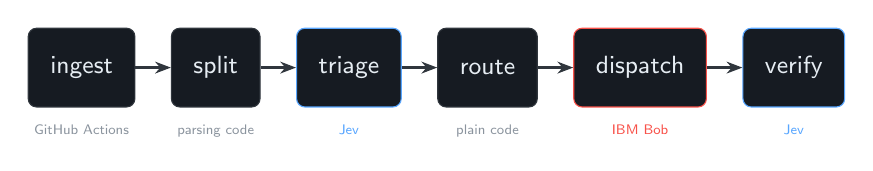
\begin{tikzpicture}[x=1cm,y=1cm,
    chip/.style={draw=hair, fill=panel, rounded corners=3pt,
                 minimum height=1.0cm, inner xsep=0.28cm, font=\small, text=ink},
    lbl/.style={font=\tiny, text=muted, inner sep=2pt},
    arr/.style={-{Stealth[length=2mm]}, hair, line width=0.9pt}]
  \node[chip]                                     (i) at (0,0) {ingest};
  \node[chip, right=0.45cm of i]                  (s) {split};
  \node[chip, right=0.45cm of s, draw=infra]      (t) {triage};
  \node[chip, right=0.45cm of t]                  (r) {route};
  \node[chip, right=0.45cm of r, draw=regression] (d) {dispatch};
  \node[chip, right=0.45cm of d, draw=infra]      (v) {verify};
  \foreach \a/\b in {i/s,s/t,t/r,r/d,d/v}{\draw[arr] (\a) -- (\b);}
  \node[lbl, below=0.14cm of i] {GitHub Actions};
  \node[lbl, below=0.14cm of s] {parsing code};
  \node[lbl, below=0.14cm of t, text=infra] {Jev};
  \node[lbl, below=0.14cm of r] {plain code};
  \node[lbl, below=0.14cm of d, text=regression] {IBM Bob};
  \node[lbl, below=0.14cm of v, text=infra] {Jev};
\end{tikzpicture}

\vspace{0.9cm}
\begin{columns}[T]
\begin{column}{0.30\textwidth}\small
\textcolor{muted}{Splitting a log is a}\\\textcolor{ink}{parsing problem.}\\
\textcolor{muted}{So code does it.}
\end{column}
\begin{column}{0.33\textwidth}\small
\textcolor{muted}{What a failure \emph{is} is}\\\textcolor{ink}{judgement under uncertainty.}\\
\textcolor{muted}{So Jev does it.}
\end{column}
\begin{column}{0.30\textwidth}\small
\textcolor{muted}{What to \emph{do} is}\\\textcolor{ink}{policy.}\\
\textcolor{muted}{So readable code does it.}
\end{column}
\end{columns}
\end{frame}

% ---------------------------------------------------------------- split
\begin{frame}{Split}{One unit per failing test or step --- no model involved}
\vspace{0.1cm}
\begin{columns}[T]
\begin{column}{0.50\textwidth}
\begin{itemize}\setlength\itemsep{0.45em}
  \item pytest, jest/vitest, go test, plus a step-level fallback
  \item Timestamps and ANSI colour stripped
  \item Signatures are \emph{scored}, not first-matched
  \item \textcolor{ink}{The same failure across six matrix legs collapses into one unit}
\end{itemize}
\vspace{0.3em}
{\footnotesize\textcolor{muted}{Six Python versions failing one lint hook is one
bug --- reporting it six times would spend six agents on a single fix.}}
\end{column}
\begin{column}{0.46\textwidth}
\term[0.95\columnwidth]{%
\textcolor{muted}{\# pydantic/pydantic, a real run}\\[0.4em]
before: 7 units\\
after:\ \ 2 units\\[0.6em]
\textcolor{config}{config} \ \ \ 64\%\ \ human\ \ \textcolor{muted}{x6 jobs}\\
\ \ \ \ Lint...........Failed\\[0.4em]
\textcolor{flaky}{flaky} \ \ \ \ 46\%\ \ human}
\end{column}
\end{columns}
\end{frame}

% ---------------------------------------------------------------- jev
\begin{frame}{Triage}{One state, three typed questions, calibrated probabilities}
\vspace{0.3cm}
\begin{columns}[T]
\begin{column}{0.46\textwidth}
\term[0.95\columnwidth]{%
POST /v1/systemone\\[0.5em]
\textcolor{infra}{category} \ \ \ \ Choice\\
\ \ regression | flaky | infra\\
\ \ | dependency | config\\[0.5em]
\textcolor{infra}{caused\_by\_pr} Noul\\
\ \ did this PR's files cause it?\\[0.5em]
\textcolor{infra}{severity} \ \ \ \ Score\\
\ \ cosmetic .. release blocker}
\end{column}
\begin{column}{0.50\textwidth}
\begin{itemize}\setlength\itemsep{0.5em}
  \item The state is the log excerpt, the files the traceback named, and the PR diff summary
  \item Jev returns \textcolor{ink}{probabilities, not prose} --- so code can branch on them
  \item Attribution is measured over \emph{source} files, not the test file
\end{itemize}
\vspace{0.2em}
{\footnotesize\textcolor{muted}{A failing test always names its own file, so counting
it would dilute the signal identically on every unit.}}
\end{column}
\end{columns}
\end{frame}

% ---------------------------------------------------------------- route
\begin{frame}{Route}{Confidence gates automation}
\vspace{0.35cm}
\centering
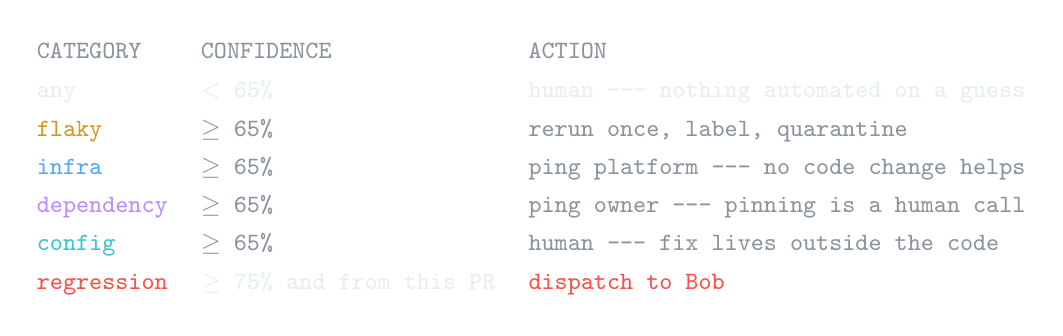
\begin{tikzpicture}[x=1cm,y=1cm]
  \node[anchor=north west, font=\ttfamily\small, text=muted] at (0,0)
  {\begin{tabular}{@{}l l l@{}}
    \textcolor{muted}{CATEGORY} & \textcolor{muted}{CONFIDENCE} & \textcolor{muted}{ACTION}\\[0.35em]
    \textcolor{ink}{any}        & \textcolor{ink}{$<$ 65\%}  & \textcolor{ink}{human --- nothing automated on a guess}\\[0.3em]
    \textcolor{flaky}{flaky}      & $\geq$ 65\% & rerun once, label, quarantine\\[0.3em]
    \textcolor{infra}{infra}      & $\geq$ 65\% & ping platform --- no code change helps\\[0.3em]
    \textcolor{dependency}{dependency} & $\geq$ 65\% & ping owner --- pinning is a human call\\[0.3em]
    \textcolor{config}{config}     & $\geq$ 65\% & human --- fix lives outside the code\\[0.3em]
    \textcolor{regression}{regression} & \textcolor{ink}{$\geq$ 75\% and from this PR} & \textcolor{regression}{dispatch to Bob}\\
  \end{tabular}};
\end{tikzpicture}

\vspace{0.9cm}
{\small\textcolor{muted}{Anything TriSolver is unsure about goes where it would
have gone anyway: to a person.}}
\end{frame}

% ---------------------------------------------------------------- bob
\begin{frame}{Dispatch}{One self-contained brief per regression}
\vspace{0.1cm}
\begin{columns}[T]
\begin{column}{0.50\textwidth}
\begin{itemize}\setlength\itemsep{0.45em}
  \item The failure, the implicated files, the PR diff, and the repo's own
        \textcolor{ink}{CONTRIBUTING / runbook}
  \item Acceptance criteria stated up front --- word for word the gates the patch will face
  \item Three adapters: \texttt{cli} (headless \texttt{bob run}), \texttt{inbox}, \texttt{fixture}
  \item Units are independent, so regressions fan out one per subagent
\end{itemize}
\end{column}
\begin{column}{0.46\textwidth}
\term[0.95\columnwidth]{%
\textcolor{muted}{\#\# Acceptance criteria}\\[0.45em]
Rejected if it:\\
1. does not address the failure\\
2. touches unrelated files\\
3. \textcolor{regression}{deletes, skips or weakens a test}\\
4. contradicts the conventions\\[0.7em]
\textcolor{ink}{Fix the code. Do not fix the test.}}
\end{column}
\end{columns}
\end{frame}

% ---------------------------------------------------------------- verify
\begin{frame}{Verify}{Two independent checks --- either one blocks alone}
\vspace{0.5cm}
\centering
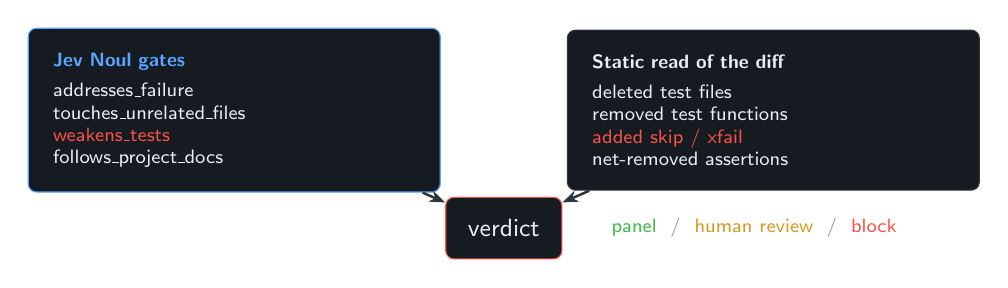
\begin{tikzpicture}[x=1cm,y=1cm,
    box/.style={draw=hair, fill=panel, rounded corners=3pt, text width=4.6cm,
                align=left, inner sep=9pt, font=\scriptsize, text=ink},
    arr/.style={-{Stealth[length=2mm]}, hair, line width=0.9pt}]
  \node[box, draw=infra] (j) at (0,0)
    {\textcolor{infra}{\textbf{Jev Noul gates}}\\[0.4em]
     addresses\_failure\\ touches\_unrelated\_files\\
     \textcolor{regression}{weakens\_tests}\\ follows\_project\_docs};
  \node[box, right=1.6cm of j] (s)
    {\textcolor{ink}{\textbf{Static read of the diff}}\\[0.4em]
     deleted test files\\ removed test functions\\
     \textcolor{regression}{added skip / xfail}\\ net-removed assertions};
  \node[draw=regression, fill=panel, rounded corners=3pt, below=1.1cm of $(j)!0.5!(s)$,
        inner sep=8pt, font=\small, text=ink] (v) {verdict};
  \draw[arr] (j) -- (v); \draw[arr] (s) -- (v);
  \node[font=\scriptsize, text=muted, right=0.5cm of v, align=left]
    {\textcolor{good}{panel} \ / \ \textcolor{flaky}{human review} \ / \ \textcolor{regression}{block}};
\end{tikzpicture}

\vspace{0.7cm}
{\small\textcolor{muted}{A novel cheat the regex misses is still caught by the model.
A model having a bad day still cannot wave through a deleted test.}}
\end{frame}

% ---------------------------------------------------------------- the moment
\begin{frame}{The demo moment}{The agent deleted the failing test}
\vspace{0.35cm}
\centering
\term[0.86\textwidth]{%
\textcolor{regression}{\textbf{BLOCK}} \ \ \ \ \ \ test\_discount\_applied\\[0.8em]
\ \ addresses\_failure \ \ \ \ \ \ \ 0.15 \ \textcolor{regression}{\#\#\#.................}\\
\ \ touches\_unrelated\_files \ 0.01 \ \textcolor{good}{....................}\\
\ \ \textcolor{regression}{weakens\_tests} \ \ \ \ \ \ \ \ \ \ \ 0.95 \ \textcolor{regression}{\#\#\#\#\#\#\#\#\#\#\#\#\#\#\#\#\#\#\#.}\\
\ \ follows\_project\_docs \ \ \ 0.25 \ \textcolor{regression}{\#\#\#\#\#...............}\\[0.7em]
\ \ static check \ \ \ \ removed test(s): test\_discount\_applied\\
\ \ files touched \ \ \ tests/test\_pricing.py\\[0.7em]
\ \ \textcolor{regression}{BLOCKED by static check} \ \ \textcolor{regression}{BLOCKED by Jev}\\
\ \ \textcolor{muted}{The failing test was neutralised rather than the defect fixed.}}

\vspace{0.6cm}
{\small\textcolor{muted}{Deleting the failing test is the well-known way to make CI
green. It is caught automatically, twice, by two independent mechanisms.}}
\end{frame}

% ---------------------------------------------------------------- real run
\begin{frame}{A real run}{Self-hosted runner, one build, five kinds of failure}
\vspace{0.3cm}
\centering
\term[0.92\textwidth]{%
\ \ CATEGORY \ \ \ \ \ \ CONF \ \ \ PR \ \ SEVERITY \ \ \ \ \ \ \ \ ACTION\\
\ \ \textcolor{hair}{------------------------------------------------------------------------}\\
\ \ \textcolor{regression}{regression} \ \ \ \ 97\% \ \ 94\% \ \ major \ \ \ \ \ \ \ \ \ \ \textcolor{ink}{-> bob} \ \ \ \ \ \ \ \ \ test\_discount\_applied\\
\ \ \ \ \ \ \textcolor{muted}{AssertionError: assert 4977 == 4978}\\[0.35em]
\ \ \textcolor{dependency}{dependency} \ \ \ \ 97\% \ \ 12\% \ \ major \ \ \ \ \ \ \ \ \ \ ping deps\\
\ \ \textcolor{config}{config} \ \ \ \ \ \ \ \ 97\% \ \ 12\% \ \ minor \ \ \ \ \ \ \ \ \ \ human\\
\ \ \textcolor{infra}{infra} \ \ \ \ \ \ \ \ \ 97\% \ \ 12\% \ \ minor \ \ \ \ \ \ \ \ \ \ ping infra\\
\ \ \textcolor{flaky}{flaky} \ \ \ \ \ \ \ \ \ 51\% \ \ 12\% \ \ minor \ \ \ \ \ \ \ \ \ \ human \ \textcolor{muted}{(below floor)}\\[0.6em]
\ \ 5 failure unit(s): 1 -> bob, 2 human, 1 ping deps, 1 ping infra}

\vspace{0.55cm}
{\small\textcolor{muted}{\texttt{usernotfound-101/testrepobob} --- a real PR, real
GitHub Actions logs, four jobs red. Four routed away from Bob.}}
\end{frame}

% ---------------------------------------------------------------- bob real
\begin{frame}{Bob fixes the one that was real}{And the gates check it before a human sees it}
\vspace{0.25cm}
\begin{columns}[T]
\begin{column}{0.47\textwidth}
\term[0.95\columnwidth]{%
\textcolor{muted}{bob run --mode agent}\\
\textcolor{muted}{task 3ed0eeca...\ \ 149s\ \ \$0.40}\\
\textcolor{muted}{13 tool calls}\\[0.8em]
--- a/src/storefront/pricing.py\\
+++ b/src/storefront/pricing.py\\
\textcolor{regression}{-\ \ \ \ return int(total)}\\
\textcolor{good}{+\ \ \ \ return round(total)}}
\end{column}
\begin{column}{0.49\textwidth}
\term[0.95\columnwidth]{%
\textcolor{good}{\textbf{SURFACE}} \ \ \ test\_discount\_applied\\[0.7em]
addresses\_failure \ \ \ \ \ \ \ 0.88\\
touches\_unrelated\_files \ 0.01\\
weakens\_tests \ \ \ \ \ \ \ \ \ \ \ 0.04\\
follows\_project\_docs \ \ \ 0.82\\[0.6em]
\textcolor{muted}{static: no test weakening}\\
\textcolor{muted}{files: src/storefront/pricing.py}}
\end{column}
\end{columns}
\vspace{0.55cm}
{\small\textcolor{muted}{CONTRIBUTING.md says money is integer cents and rounding
happens once, at the end. Bob's fix matches that rule --- and the test suite passes.}}
\end{frame}

% ---------------------------------------------------------------- limits
\begin{frame}{What is proven, and what is not}{}
\vspace{0.3cm}
\begin{columns}[T]
\begin{column}{0.47\textwidth}
{\textcolor{good}{\textbf{Validated}}}
\begin{itemize}\setlength\itemsep{0.4em}\small
  \item Live ingestion against real failed runs in \texttt{psf/requests},
        \texttt{pydantic/pydantic}, \texttt{urllib3/urllib3}, \texttt{encode/httpx}
  \item A purpose-built sandbox on a self-hosted runner: five categories, one build
  \item Bob's real patch cleared all four gates; the suite passes
  \item 75 tests
\end{itemize}
\end{column}
\begin{column}{0.47\textwidth}
{\textcolor{flaky}{\textbf{Not yet}}}
\begin{itemize}\setlength\itemsep{0.4em}\small
  \item \textcolor{ink}{Jev runs in a labelled offline simulator} --- no API key yet.
        Thresholds are tuned for real calibrated probabilities
  \item That is why the flaky unit scored 51\% and fell to a human
  \item Subagent fan-out is built but undemonstrated: this run had one regression
  \item No watsonx.ai or watsonx Orchestrate
\end{itemize}
\end{column}
\end{columns}
\end{frame}

% ---------------------------------------------------------------- close
\begin{frame}[plain]
\begin{tikzpicture}[remember picture,overlay,x=1cm,y=1cm]
  \fill[regression] (0.72,3.7) rectangle (3.5,3.81);
  \node[anchor=north west, ink, font=\fontsize{30}{34}\bfseries, text width=12cm] at (0.66,3.3)
    {Sort the red build.\\Fix only what is real.\\Check the fix.};
  \node[anchor=north west, muted, font=\small] at (0.68,-1.35)
    {TriSolver \ \ $\cdot$ \ \ Jev for judgement \ \ $\cdot$ \ \ IBM Bob for the fix};
\end{tikzpicture}
\end{frame}

\end{document}
